%\section{Verification of the method}\label{Sec:App}
%\deleted{This appendix devotes to a verification of our implementation of the present phase field method for CO$_2$ fracturing. To this end, we present three examples with exact or otherwise trusted solutions to study how our outputs are in accordance with the analytical solutions and other works.}

\subsection{Single-edge-notched tension test}
{First, following an example motivated by Miehe \emph{et al.}~\cite{miehe2010phase},} we %\deleted{first} 
investigate a square plate with a horizontal {initial} crack at the middle height starting from the left end and ending at the plate center. The geometric setup is depicted in Figure \ref{Fig:Notched_geometry}. To capture the crack pattern properly, the mesh is refined in areas where the crack is expected to propagate, i.e., in the center strip of the specimen. In effect, for a discretization with 105,352 standard $P_1$ elements, an effective element size of $h\approx 5\times 10^{-3}$ mm is obtained in the critical zone. The specimen is under a direct tension test, in which a monotonically increasing displacement with constant increments $\Delta\bm{u}=6 \times 10^{-5}$ mm is imposed on the top edge while the bottom edge is fixed. In this example, the evolution is simulated for 100 uniform time steps so that a final deformation of $6\times 10^{-3}$ mm is reached. We will adopt the values of the material parameters given in Table \ref{Tab:Notched_input}. %\deleted{Note that all our models are implemented with the AT1 model.}
%Also, the {regularization parameter} is set to be $l=\dots~mm$.
\begin{figure}[htbp]
    \centering
    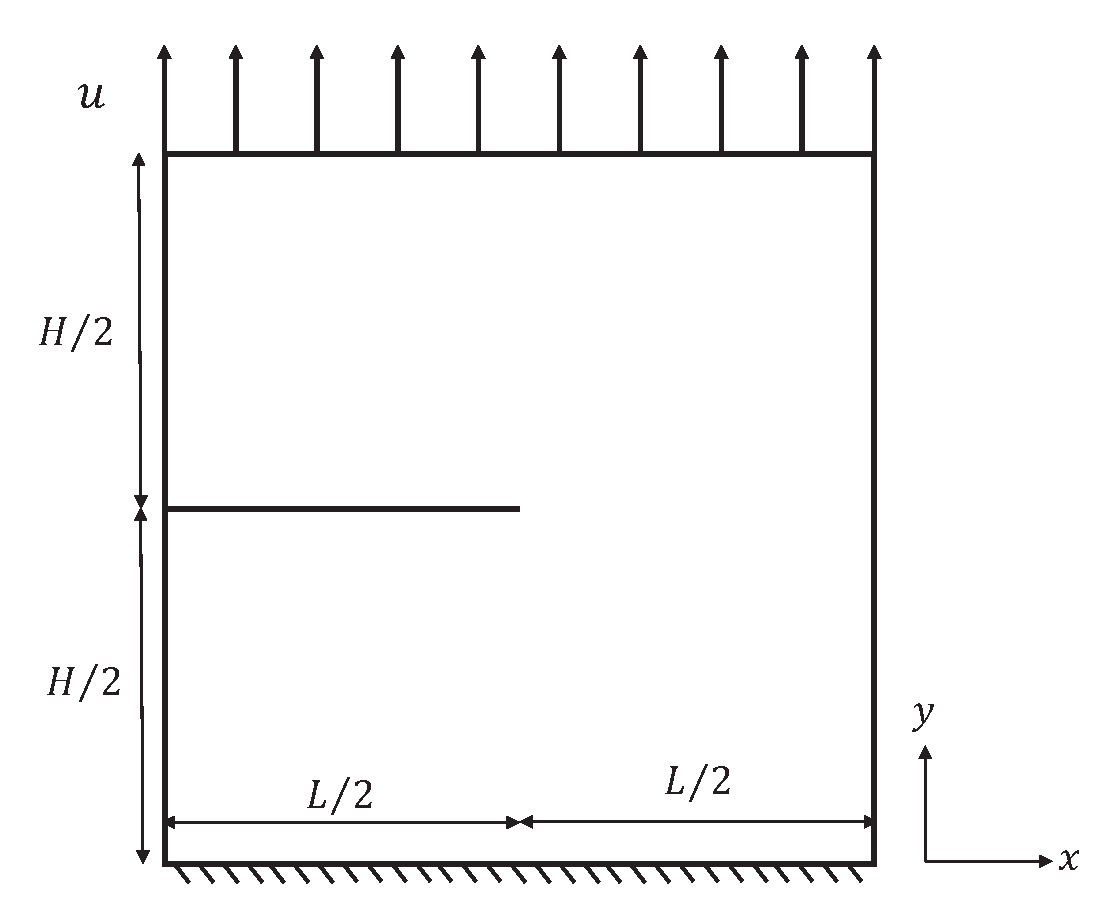
\includegraphics[width=80mm]{edgeNotch}
    \caption{Schematic of a cracked square plate (unit: mm) under a single-edge-notched tension test. 
    A monotonically increasing displacement with constant increments $\Delta\bm{u}=6\times 10^{-5}$ mm is applied on the top edge while the bottom edge is fixed.}
    \label{Fig:Notched_geometry}
\end{figure}

\begin{table}[htbp]
    \centering
    \caption{Cracked square plate under a tension test: Material parameters \cite{ambati2015review}}
    \begin{tabular}{l c c c}
    \hline 
         Parameters & symbol & unit& value \\
    \hline 
         Young's modulus & $E$ &MPa&  210$\times 10^{3}$\\
         Poisson's ratio & $\nu$ &$-$&  0.3\\
         Critical energy release rate & $g_c$ &MPa$\cdot$mm&  2.7\\
            \hline      
    \end{tabular}
    \label{Tab:Notched_input}
\end{table}

The resulting crack patterns at different stages of the deformation for two fixed regularization length scales $\ell = \ell_1 = 1\times 10^{-2}$ mm and $\ell = \ell_2=2 \times 10^{-2}$ mm are illustrated in Figure \ref{Fig:Notched_snapshots}. 
As expected, in both simulations, the fracture propagates straightforward to the end. This straight crack topology agrees well with the results in \cite{miehe2010thermodynamically}. Also as seen, the resulting crack pattern with the smaller $\ell$ looks sharper.

\begin{figure}[!htb]
    \centering
    \subfloat[]{
    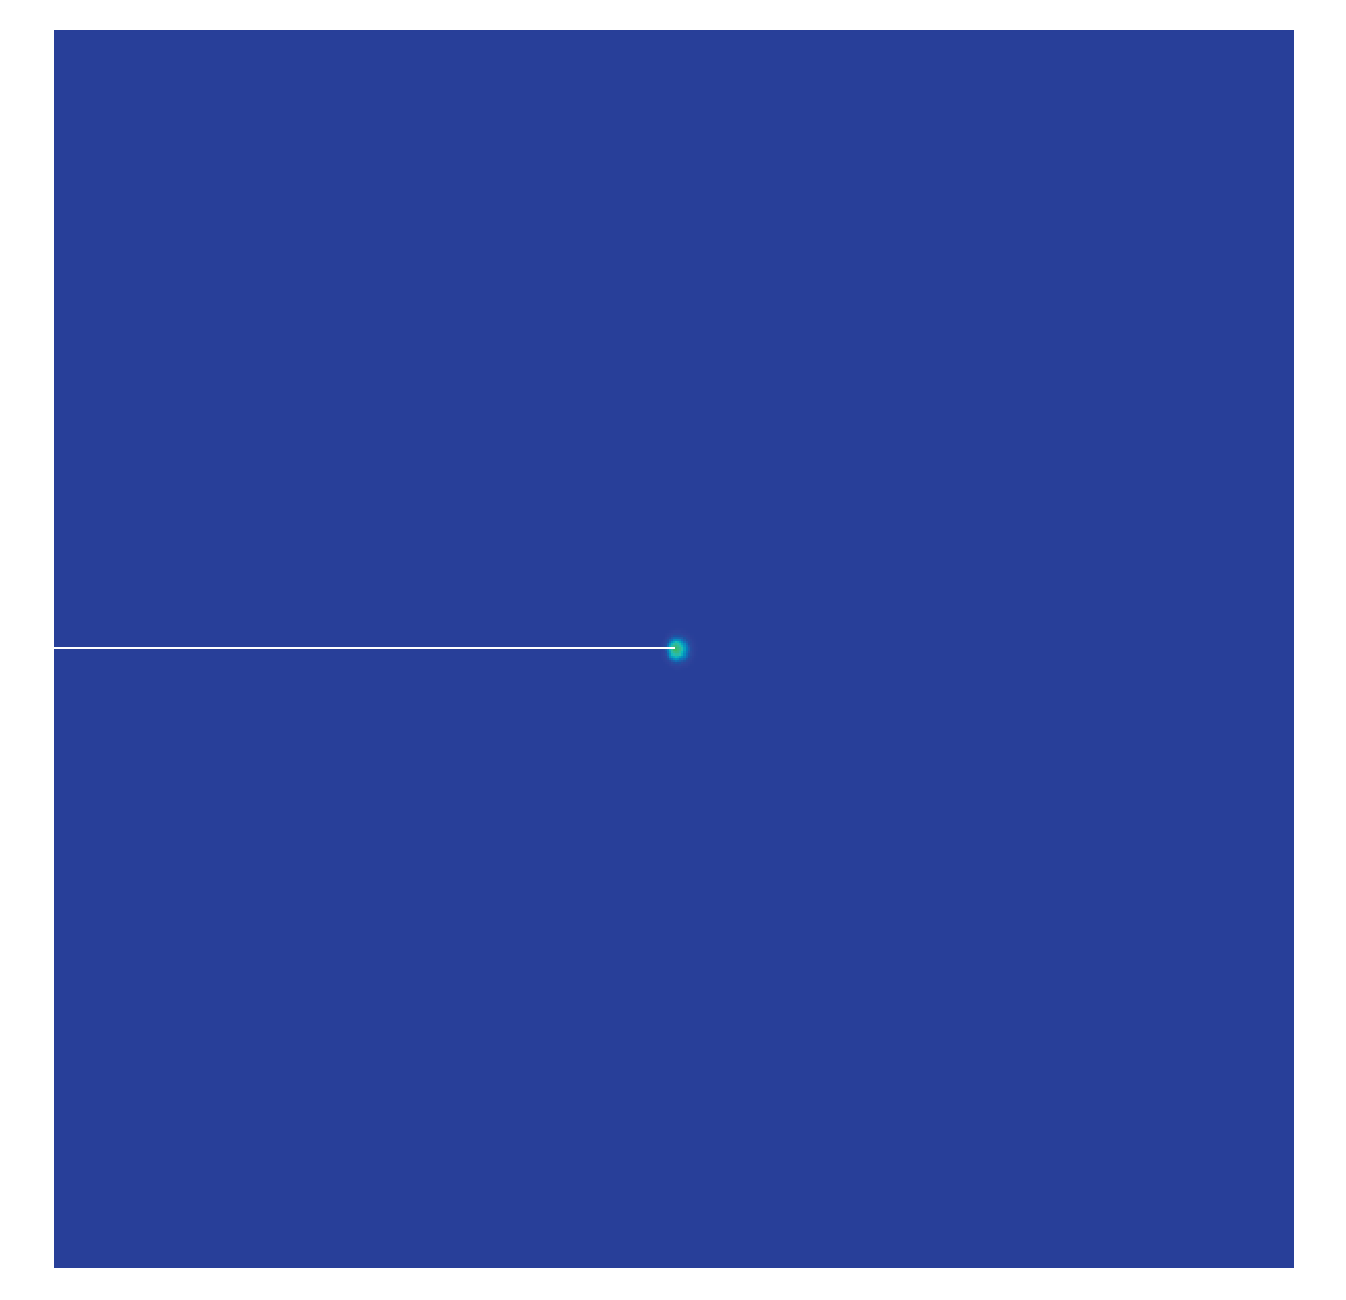
\includegraphics[width=0.43\textwidth]{snapshot_l2h_t92.eps}
    \label{Fig:Notched_lenght_scale_2h_i}}
    \subfloat[]{
    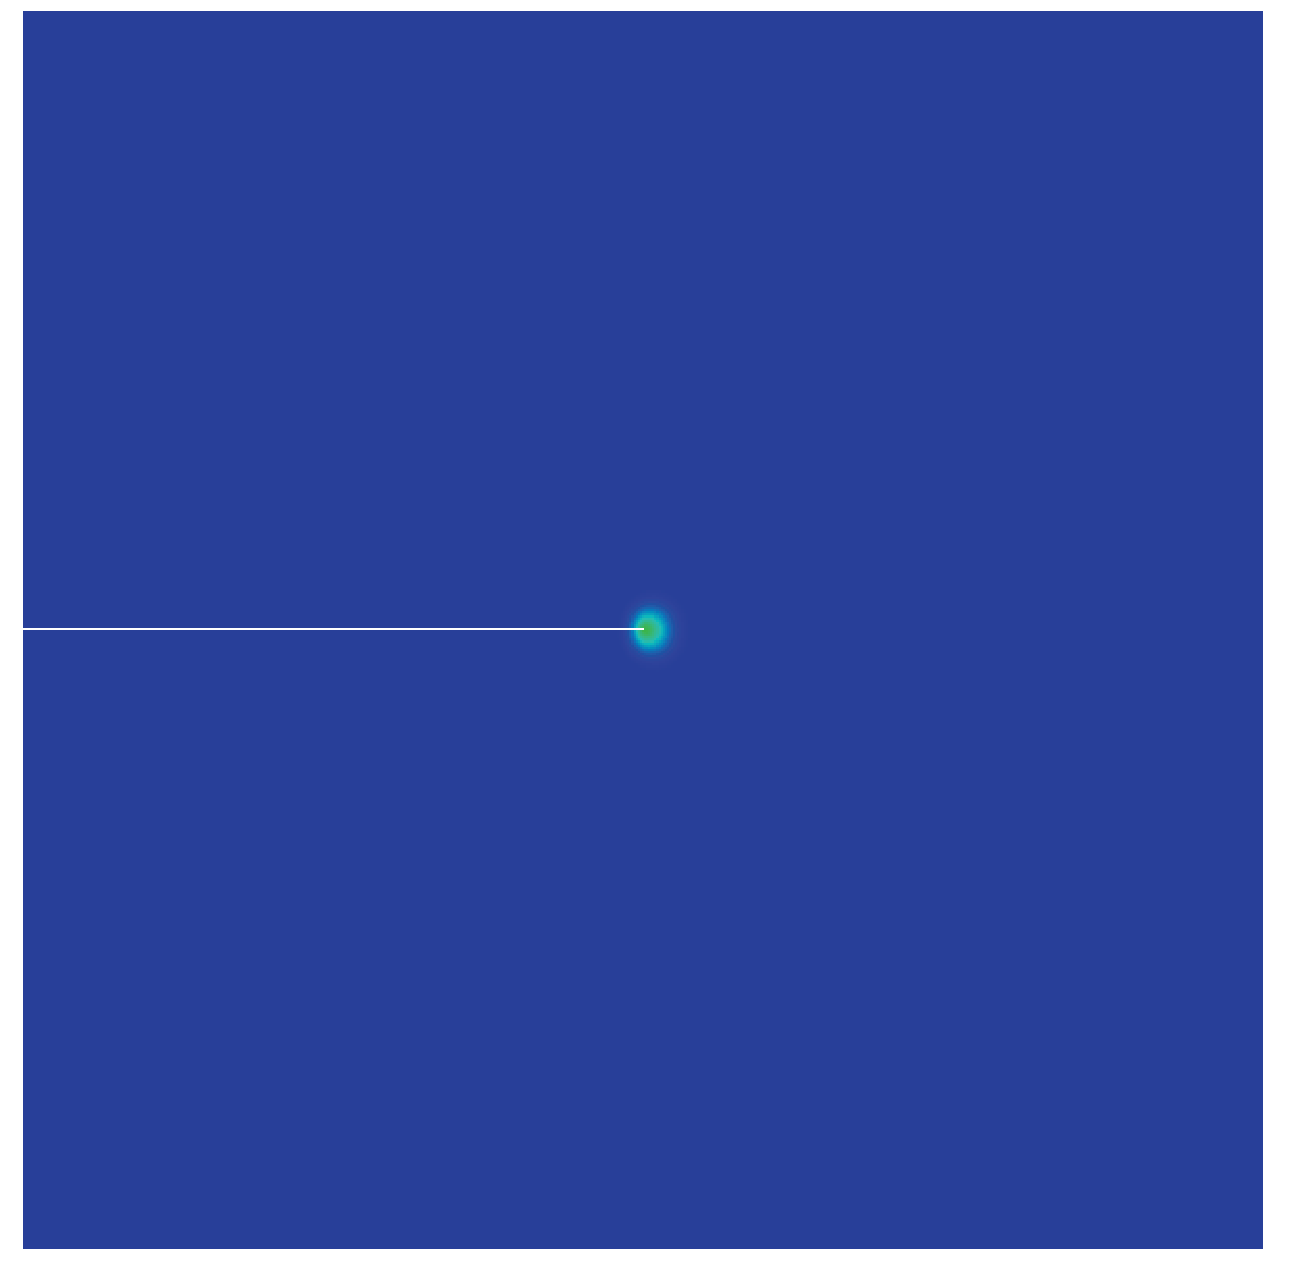
\includegraphics[width=0.437\textwidth]{snapshot_l4h_t92-eps-converted-to}
    \label{Fig:Notched_lenght_scale_4h_i}}\\
    \subfloat[]{
    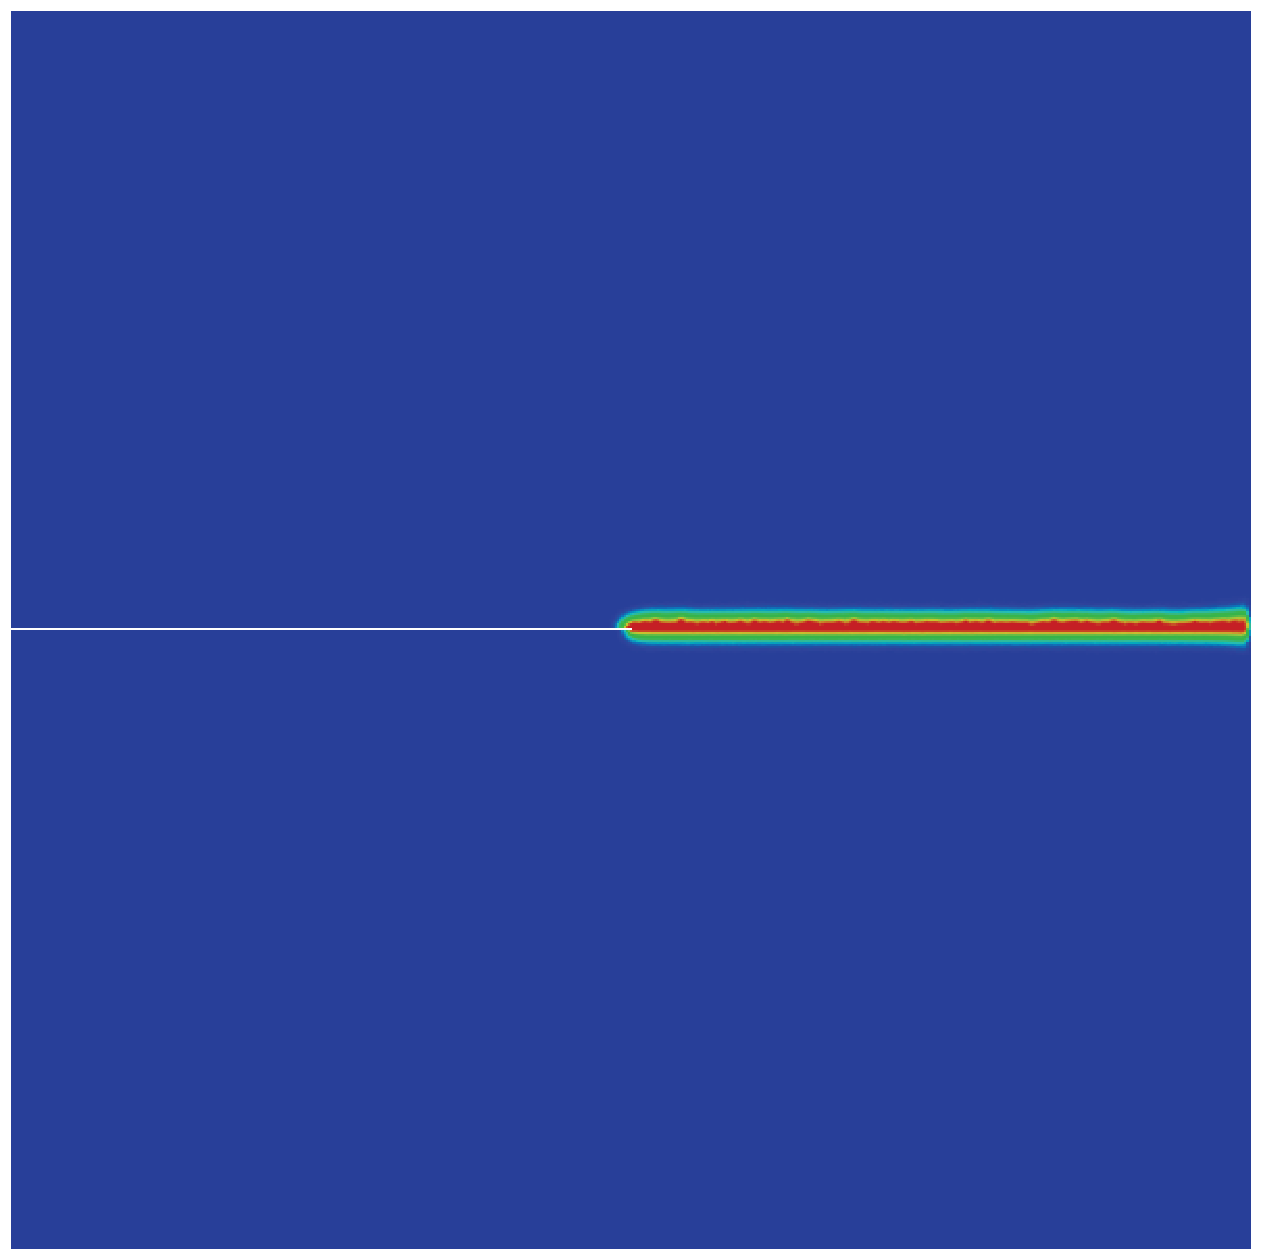
\includegraphics[width=0.43\textwidth]{snapshot_l2h_t93-eps-converted-to}
    \label{Fig:Notched_lenght_scale_2h_ii}}
    \subfloat[]{
    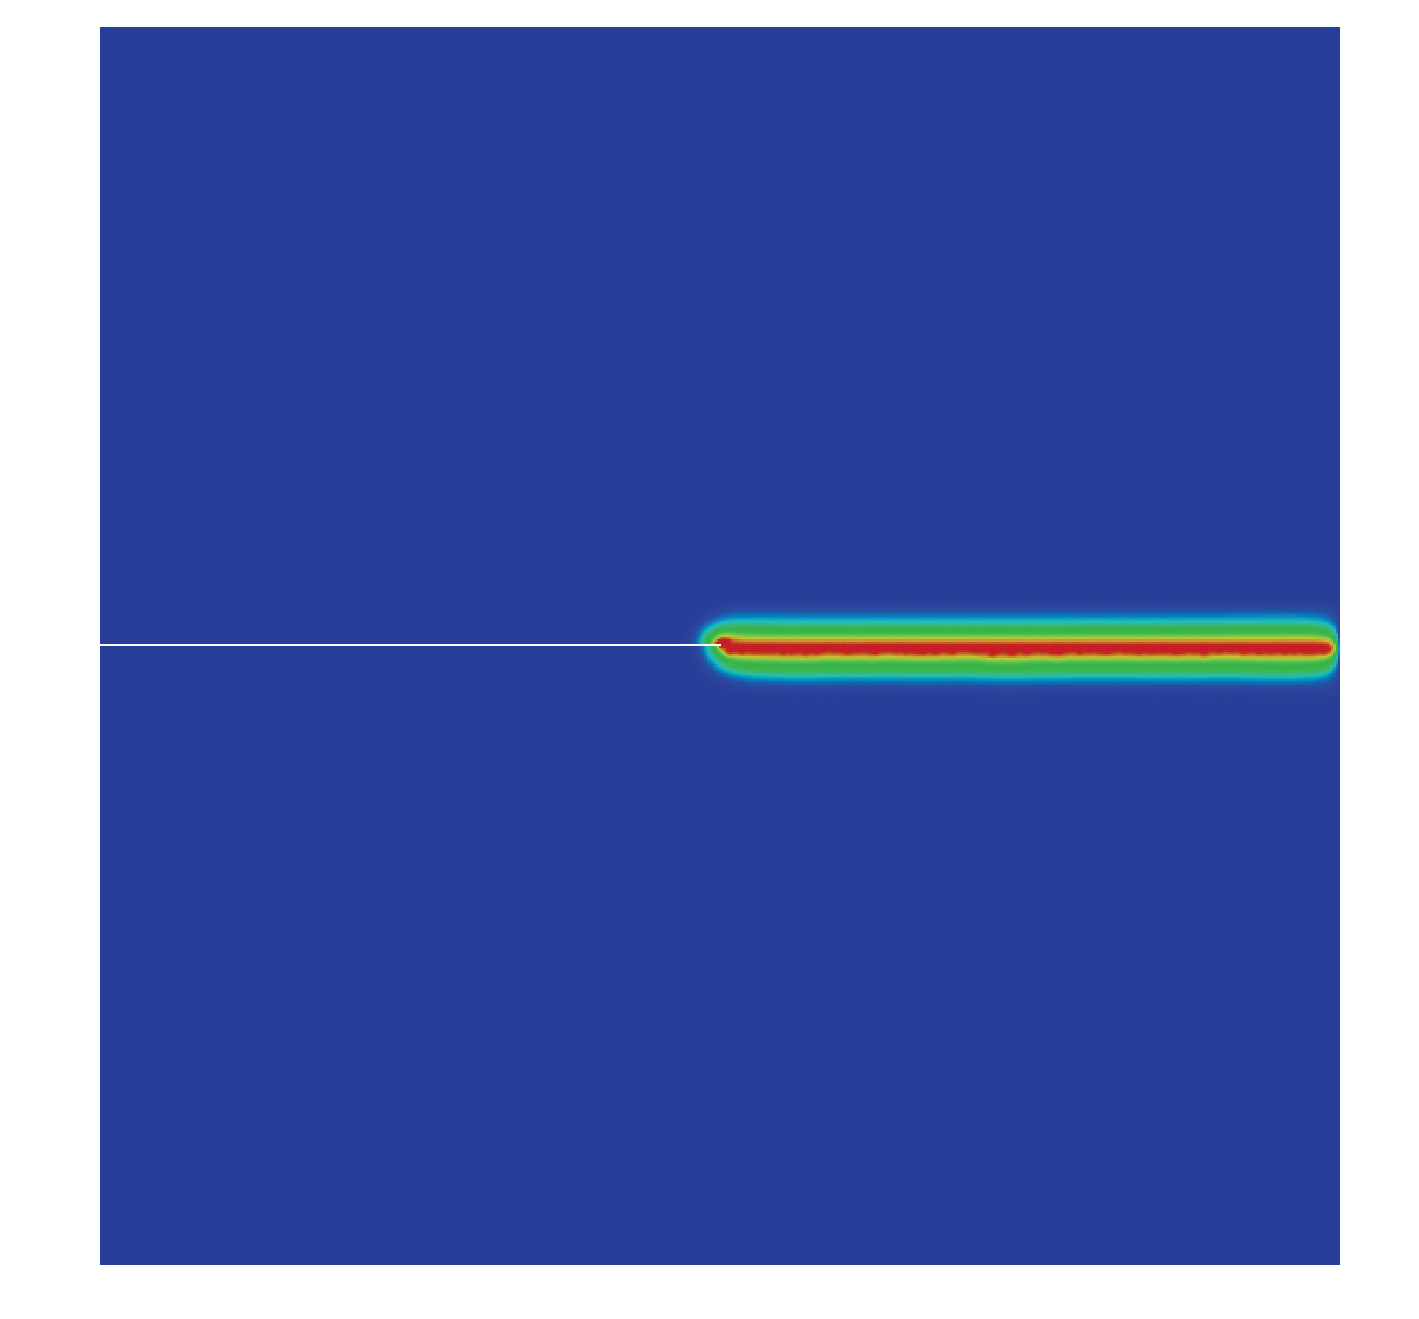
\includegraphics[width=0.43\textwidth]{snapshot_l4h_t93-eps-converted-to}
    \label{Fig:Notched_lenght_scale_4h_ii}}\\
    \subfloat[]{
    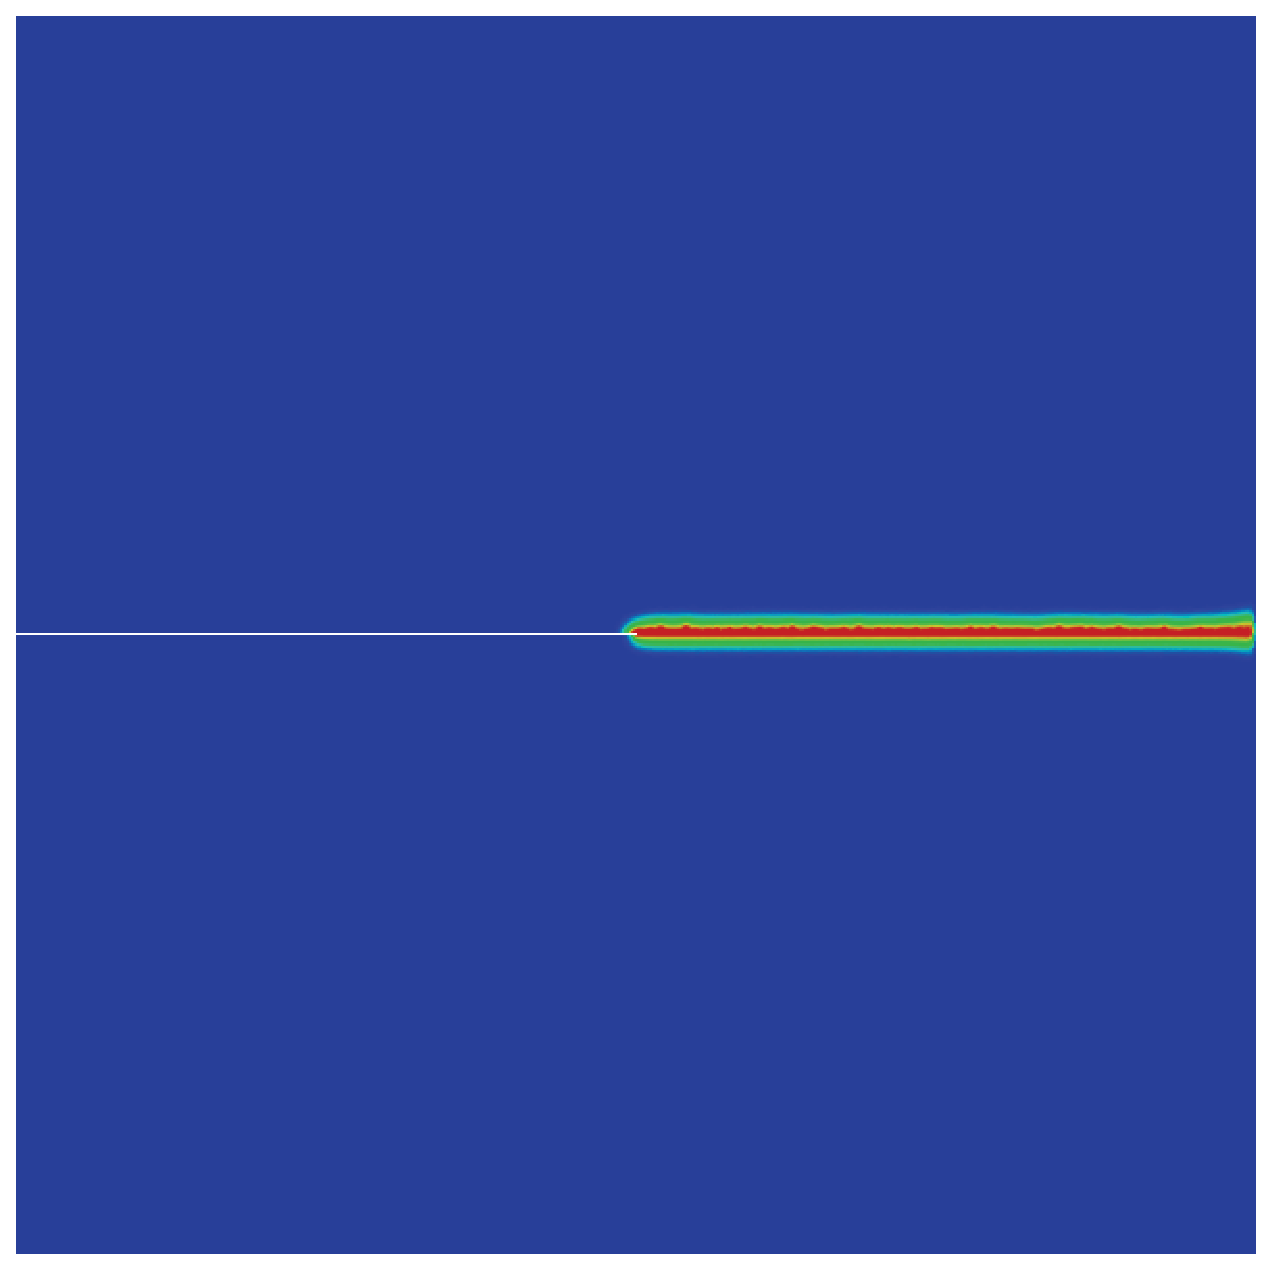
\includegraphics[width=0.43\textwidth]{snapshot_l2h_t99-eps-converted-to}
    \label{Fig:Notched_lenght_scale_2h_iii}}
    \subfloat[]{
    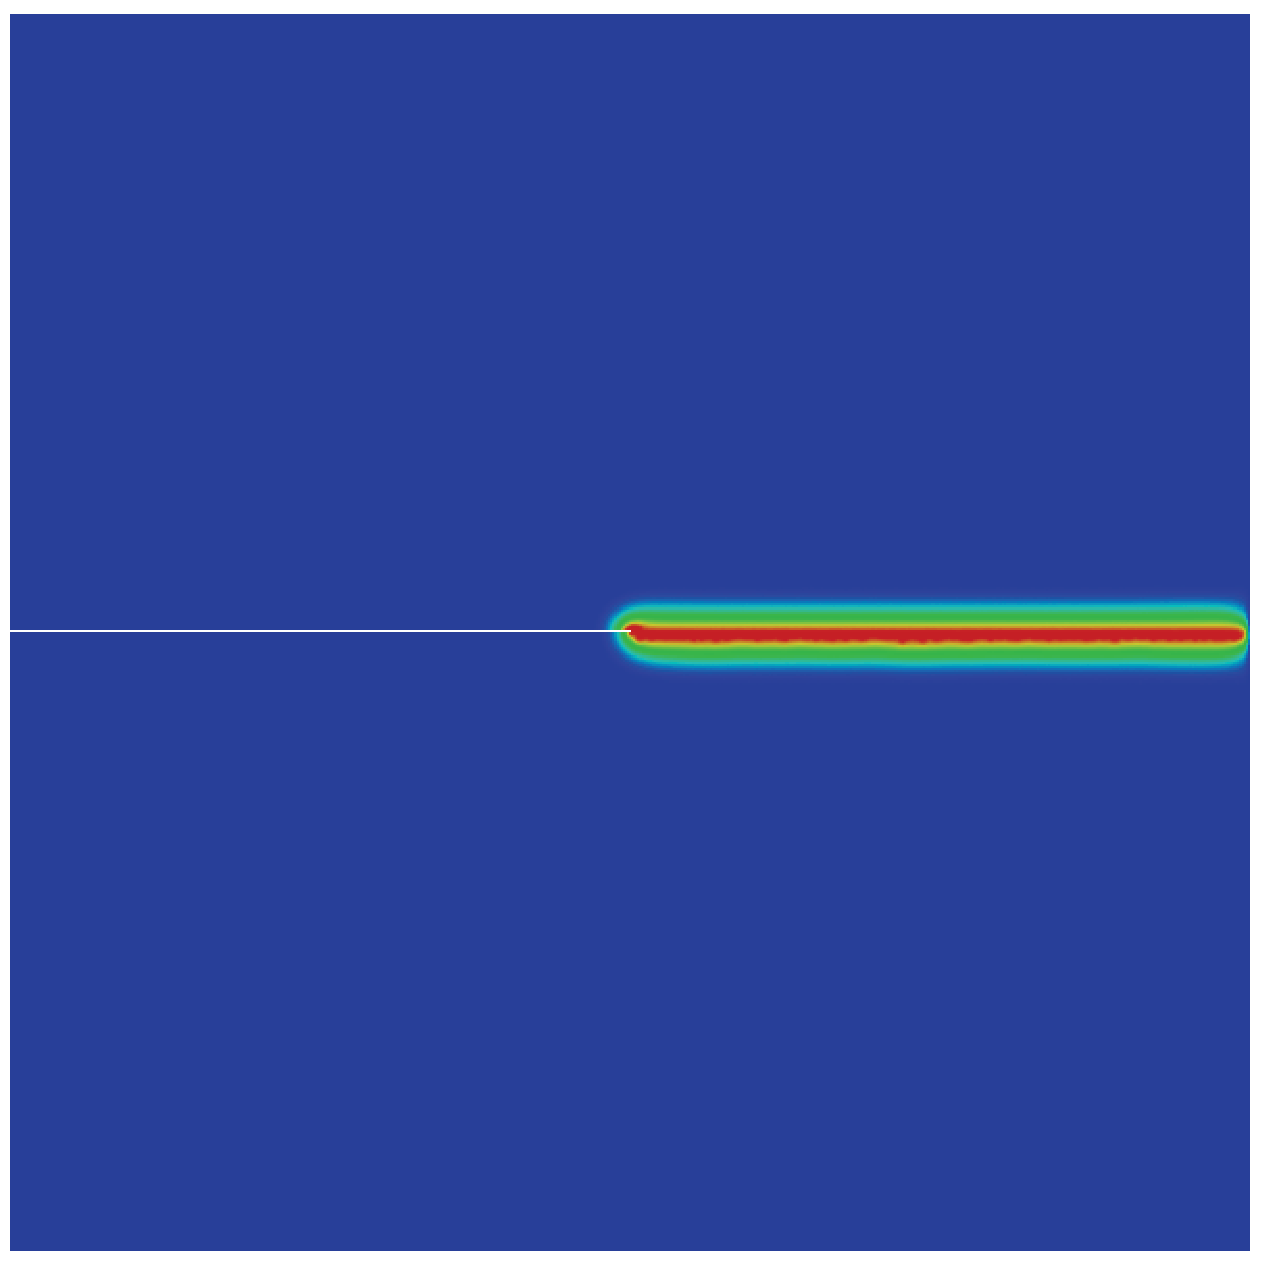
\includegraphics[width=0.43\textwidth]{snapshot_l4h_t99-eps-converted-to}
    \label{Fig:Notched_lenght_scale_4h_iii}}
	\\ 
	\subfloat{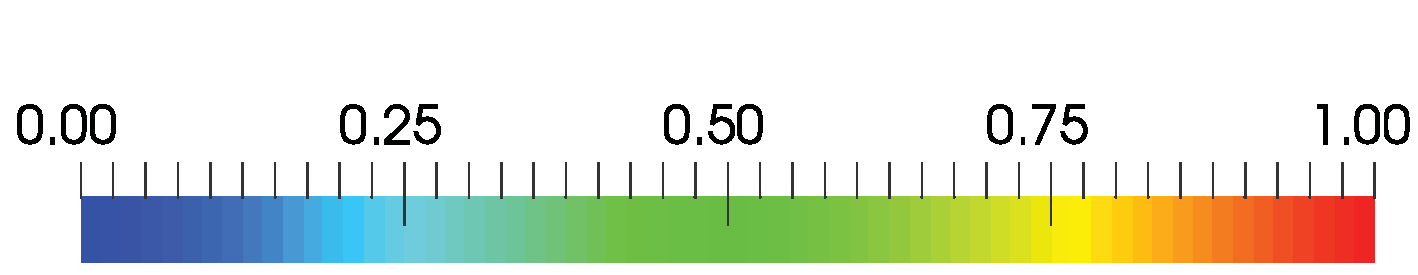
\includegraphics[width=80mm]{snapshot_COLORBAR}}

    \caption{Cracked square plate under a tension test {with two different regularization length scales $\ell=\ell_1 = 10^{-2}$ mm $\approx 2h$ (left) and $\ell=\ell_2 = 2\times 10^{-2}$ mm $\approx 4h$ (right)}. Both simulations are done with 100 uniform time steps with $\Delta\bm{u}= 6 \times 10^{-5}$ mm (See also Table \ref{Tab:Notched_input} for the input values). Phase field contours at three different stages $\bm{u}=5.52 \times 10^{-3}$ mm (\ref{Fig:Notched_lenght_scale_2h_i},\ref{Fig:Notched_lenght_scale_4h_i}), $\bm{u}=5.58 \times 10^{-3}$ mm (\ref{Fig:Notched_lenght_scale_2h_ii},\ref{Fig:Notched_lenght_scale_4h_ii}), and $\bm{u}=6 \times 10^{-3}$ mm (\ref{Fig:Notched_lenght_scale_2h_iii},\ref{Fig:Notched_lenght_scale_4h_iii}) are shown in deformed configurations with the deformations scaled. The initial cracks are explicitly imposed, so in the deformed configuration it appears as a white line. As expected, we observe a straight crack pattern in both cases.
    }
    \label{Fig:Notched_snapshots}
\end{figure}

We also output the load-deflection curves for the two setups of Figure \ref{Fig:Notched_lenght_scale}. As seen, both models will result in similar trends. Hence, the effect of $\ell$ on the response is small in this range.

\begin{figure}[htbp]
    \centering
    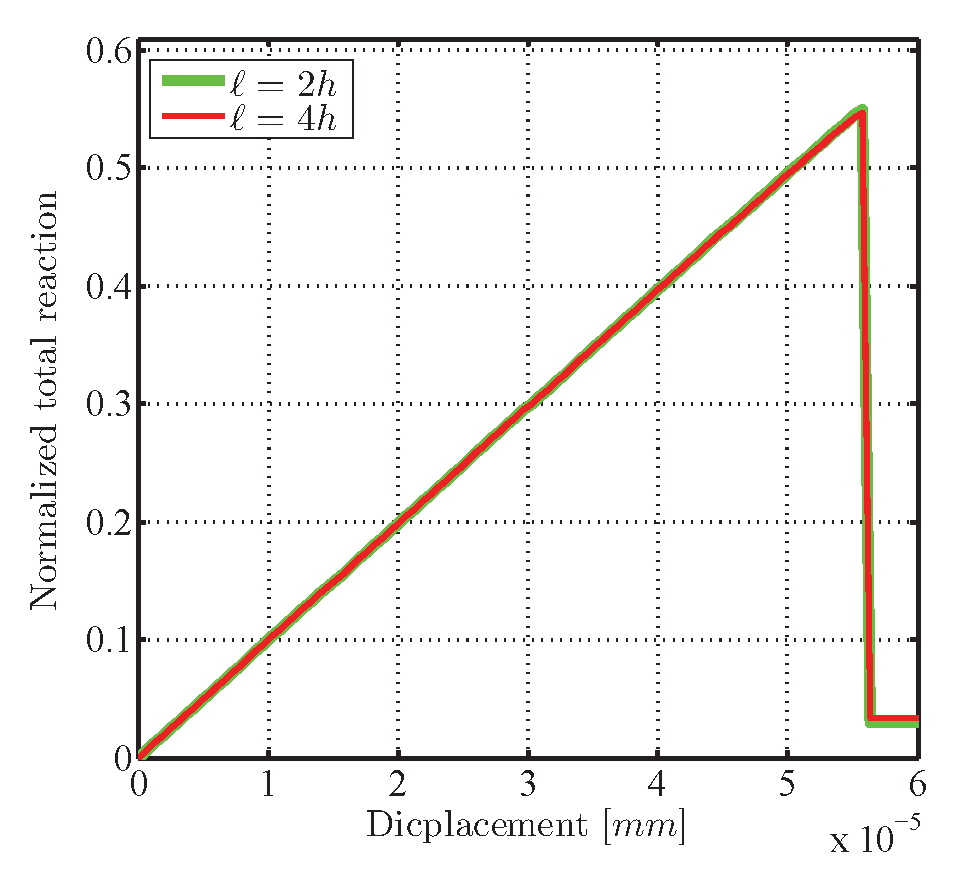
\includegraphics[width=0.6\textwidth]{Force_ELL_fracture}
    \caption{Cracked square plate under a tension test {with two different regularization length scales $\ell=\ell_1 =  10^{-2}$ mm $\approx 2h$ (red) and $\ell=\ell_2= 2\times 10^{-2}$ mm $\approx 4h$ (green)}. Load-deflection curves for both $\ell_1$ and $\ell_2$ are obtained. Both simulations are done with 100 load steps with $\Delta\bm{u}=6 \times 10^{-5}$ mm. The total reaction is normalized by the one in the case without any crack or phase field evolution. Both models give rise to similar trends so the effect of changes in $\ell$ is small within this range. Note that the reaction highly decreases at the 93rd time step where the crack starts to propagate.}
    \label{Fig:Notched_lenght_scale}
\end{figure}

%In order to point out the effects that arise due to the choice of the methods $AT1$ or $AT2$, Figure \ref{Fig:Notched_law_model} depicts the obtained load-deflection curves. Note that here we take $\ell= \added{4h}$. \added{As seen, both methods result in similar trends, although the $AT1$ method is having the higher pick value.}

%\begin{figure}[htbp]
%    \centering
 %   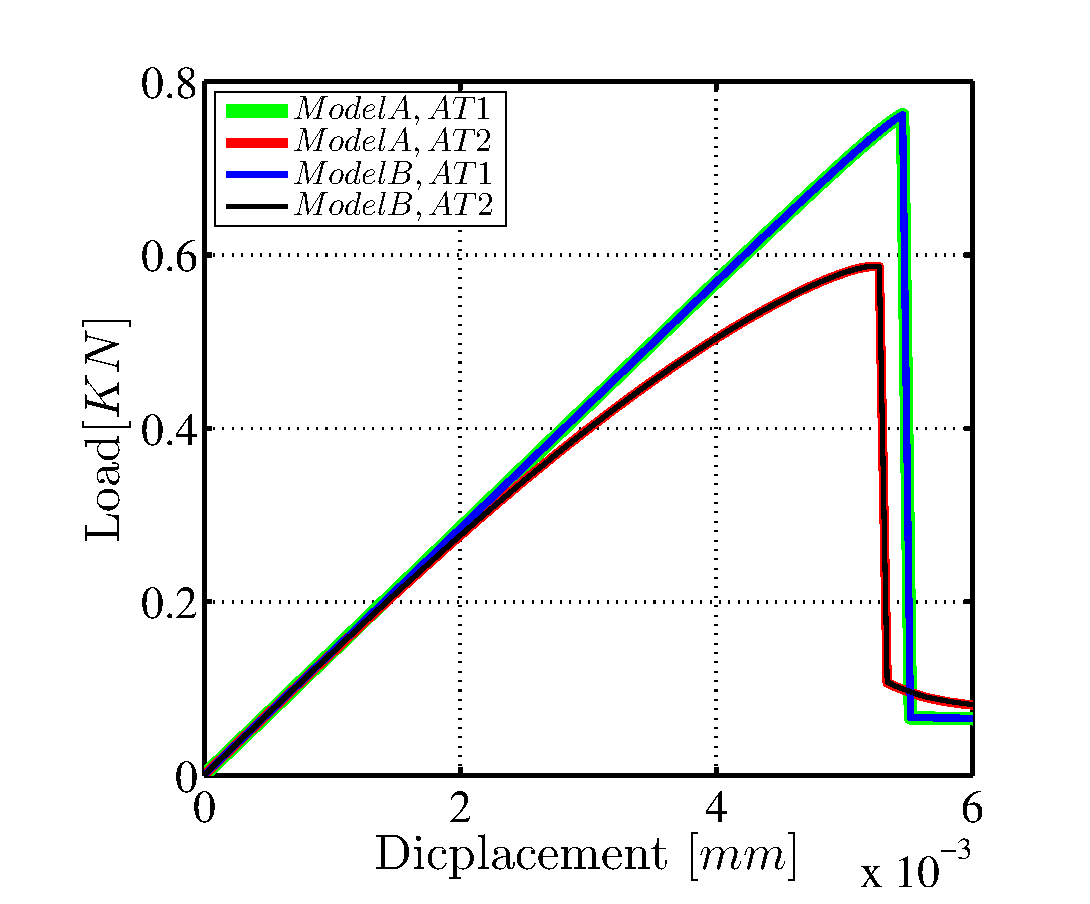
\includegraphics[width=100mm]{Force_LAW_MODEL_fracture.eps}
%    \caption{Cracked square plate under a tension test {with $\ell=\added{4h}~\text{mm}$.} Load-deflection curves for two different methods $AT1$ and $AT2$ are obtained. Both simulations are done with a number of \added{100} time steps with $\Delta\bm{u}= \added{0.006}~\text{mm}$. The total reaction is normalized by the one in the case without any crack or phase field evolution. The methods AT1 and AT2 show slightly different values while following similar trend. \added{Note that the total reaction highly decreases at the \dots-th time step where the crack starts to propagate.}}
%    \label{Fig:Notched_law_model}
%\end{figure}

\subsection{Poroelastic response of a borehole}
This example  aims to study the effect of fluid pressurization on the poroelastic response around the borehole.
It was first studied by {Detourney and Cheng} \cite{detournay1988poroelastic} (see also \cite{wang2018influence, lu2013microcrack}). Consider a plane strain hydraulic fracturing problem where there is a square plate containing a central borehole. The geometry and the loading conditions in this example are the same as Figure \ref{Fig:Gas_geometry}. The far-field \emph{in situ} stress is set to zero in this example. Note also that $d\equiv0$, i.e., there is no preexisting crack in the specimen and we do not allow for any nucleation of the fracture as the rock strength is assigned a very large value. A discretization with 28,140 standard $P_1$ elements is applied to the problem. To capture the high gradient of pressure near the borehole, the mesh is refined in that area so that an effective mesh size of $h\approx 0.15$ mm is adopted. The fluid is slightly compressible, and we set the fluid pressure in the borehole to $1$ MPa. The other material properties are prescribed according to Table \ref{Tab:Borehole_input}.

Here, the governing equation for the slightly compressible flow is written as follows \cite{detournay1988poroelastic}:
\begin{equation*}%\label{Eq:ap2}
   \begin{aligned}
        \partial_t p+ M \nabla \cdot \left(\frac{k_0}{\mu} \nabla p\right)=0
    \end{aligned}
\end{equation*}
where $M=E\left( 1-\nu\right) /[\left(1+\nu \right)\left(1-2\nu \right)]$ is called the constrained modulus.
%\todo[inline]{Vahid: Mostafa, please add the formula for $M$ in place of dots.\\Mostafa: it's added\\YS: It may be just $\lambda$ or the bulk modulus.\\Mostafa: It seems that $M $ is different from first Lame constant or bulk modulus.}
\begin{table}[htbp]
    \centering
    \caption{Poroelastic response of a borehole: Material parameters}
    \begin{tabular}{l c c c}
    \hline 
         Parameters & symbol & unit& value \\
    \hline 
         Young's modulus & $E$ &MPa&  6000\\
         Poisson's ratio & $\nu$ &$-$&  0.34\\
         Biot coefficient & $\alpha$ &$-$&  1.\\
         Permeability & $k_0$ &mm$^2$&  1$\times 10^{-12}$\\
            \hline      
    \end{tabular}
    \label{Tab:Borehole_input}
\end{table}

Figure \ref{Fig:Borehole_porepressure} shows the distribution
of pore pressure around the borehole for three values of dynamic viscosity $\mu$ at early time $t=0.1$ s. Note that the horizontal axis is $(r-r_0)/r_0$, ranging from $0$ to $0.25$ in the direction of $\theta= \pi/2$. The simulation results are then compared to the analytical solution by Detourney and Cheng \cite{detournay1988poroelastic}.

Figure \ref{Fig:Borehole_tangential_stress} depicts the effect of dynamic viscosity on the effective tangential stress in the vicinity of the borehole at early time $t=0.1$ s.%\todo{YS: Any conclusion?}

\begin{figure}[htbp]
    \centering
    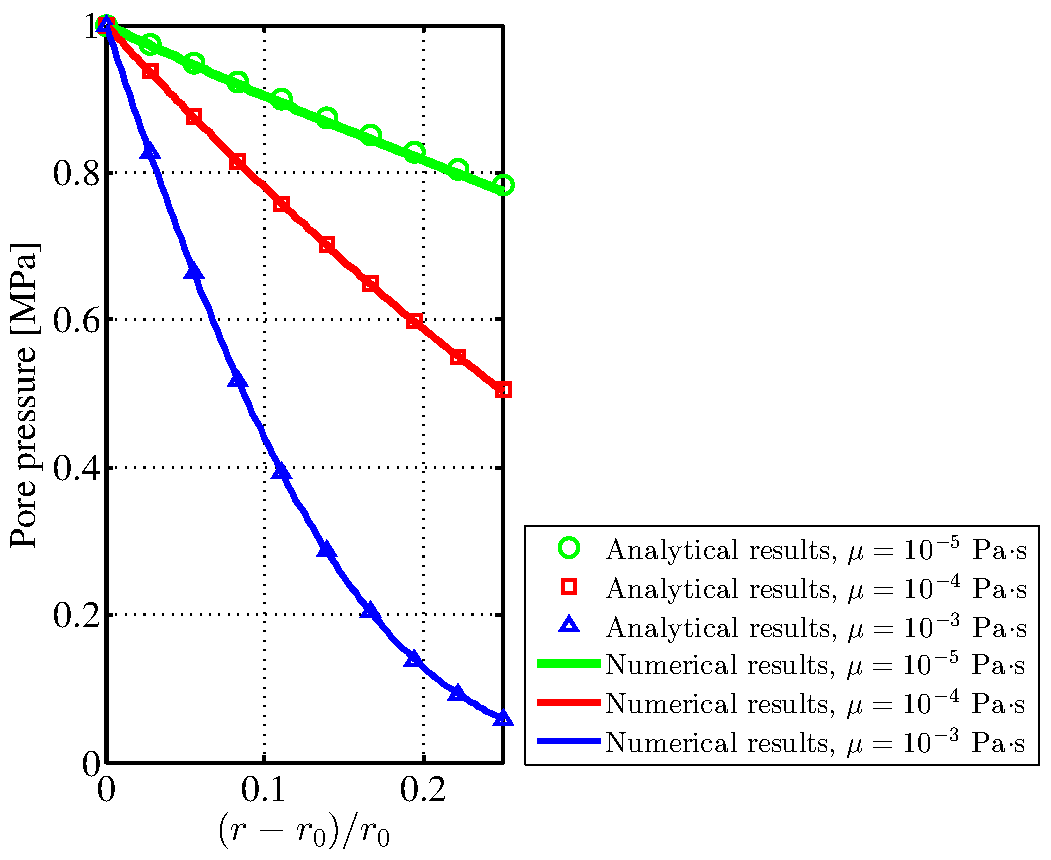
\includegraphics[width=0.8\textwidth]{verify_porepressure}
    \caption{Poroelastic response of a borehole. The distribution of pore pressure caused by fluid pressurization is shown around the borehole for three different dynamic viscosities $\mu$ at early time $t= 0.1$ s. As seen, the results are in good accordance with the analytical in \cite{detournay1988poroelastic}.}
    \label{Fig:Borehole_porepressure}
\end{figure}

\begin{figure}[htbp]
    \centering
    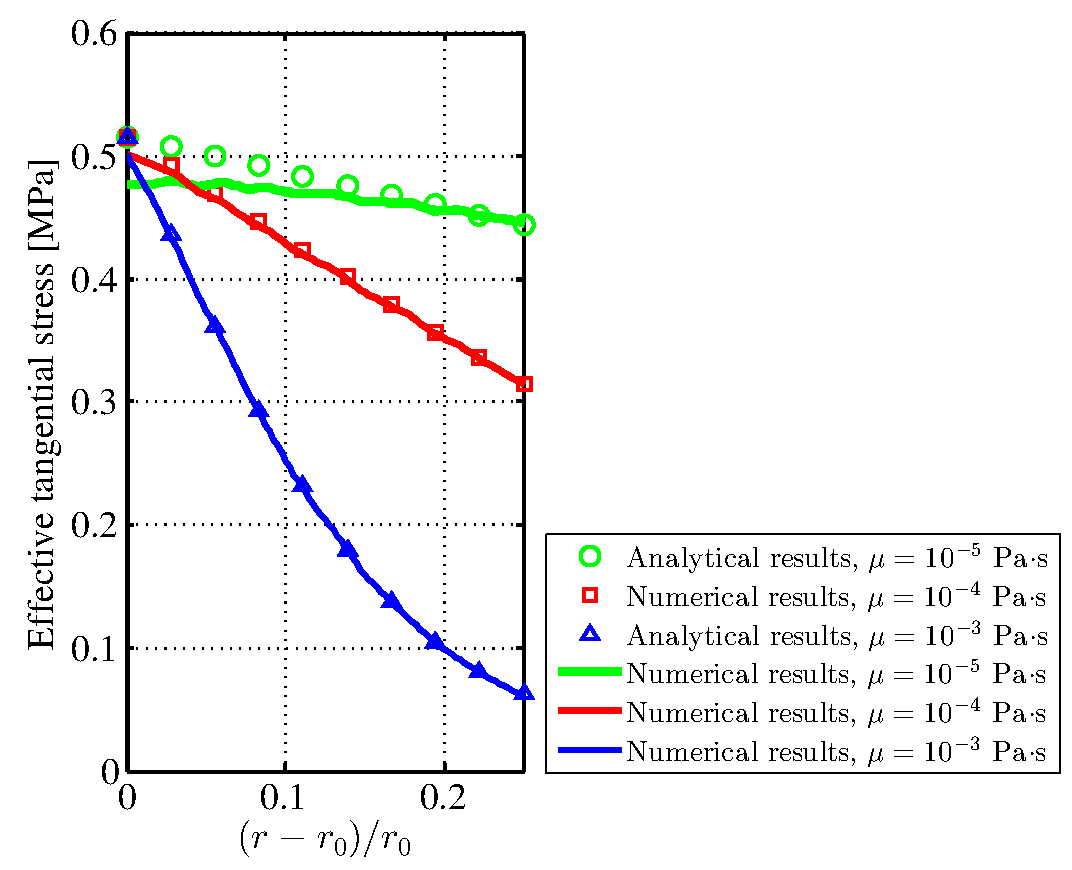
\includegraphics[width=0.8\textwidth]{verify_tangentialstress}
    \caption{Poroelastic response of a borehole. The effective tangential stress is plotted near the borehole for three different dynamic viscosities $\mu$ at early time $t=0.1$ s.}
    \label{Fig:Borehole_tangential_stress}
\end{figure}

\subsection{Computation of the crack opening displacement} \label{sec: AP-verification-opening}
We now focus on a classical problem first solved by Sneddon and Lowengrub \cite{SneddonLowengrub69} (see also \cite{bourdin2012variational}) that solves the opening displacement of a static line crack.

Consider a computational domain of $\Omega=4$ m $\times 4$ m with a preexisting line fracture of length $2a_0=0.4$ m, i.e., $\mathcal{C}=[1.8, 2.2]\times\{0\}$. To minimize the effect of the boundary conditions on the results, the domain size is much larger than the crack length ($L\gg 2a_0$).

The mechanical properties of the material are the Young's modulus $E=1000$ MPa, the Poisson's ratio $\nu=0$, and the fracture toughness $g_c=1$ MPa$\cdot$s.

We impose zero displacements on the external boundary of $\Omega$. Also we set $d=1$ on prescribed (initial) fracture and $d=0$ on the external boundary of $\Omega$. A monotonically increasing pressure is applied on the upper and lower faces of fracture with the magnitude $p=1$ MPa. Figure \ref{Fig:Sneddon_geometry} depicts the geometry and boundary conditions.

\begin{figure}
    \centering
    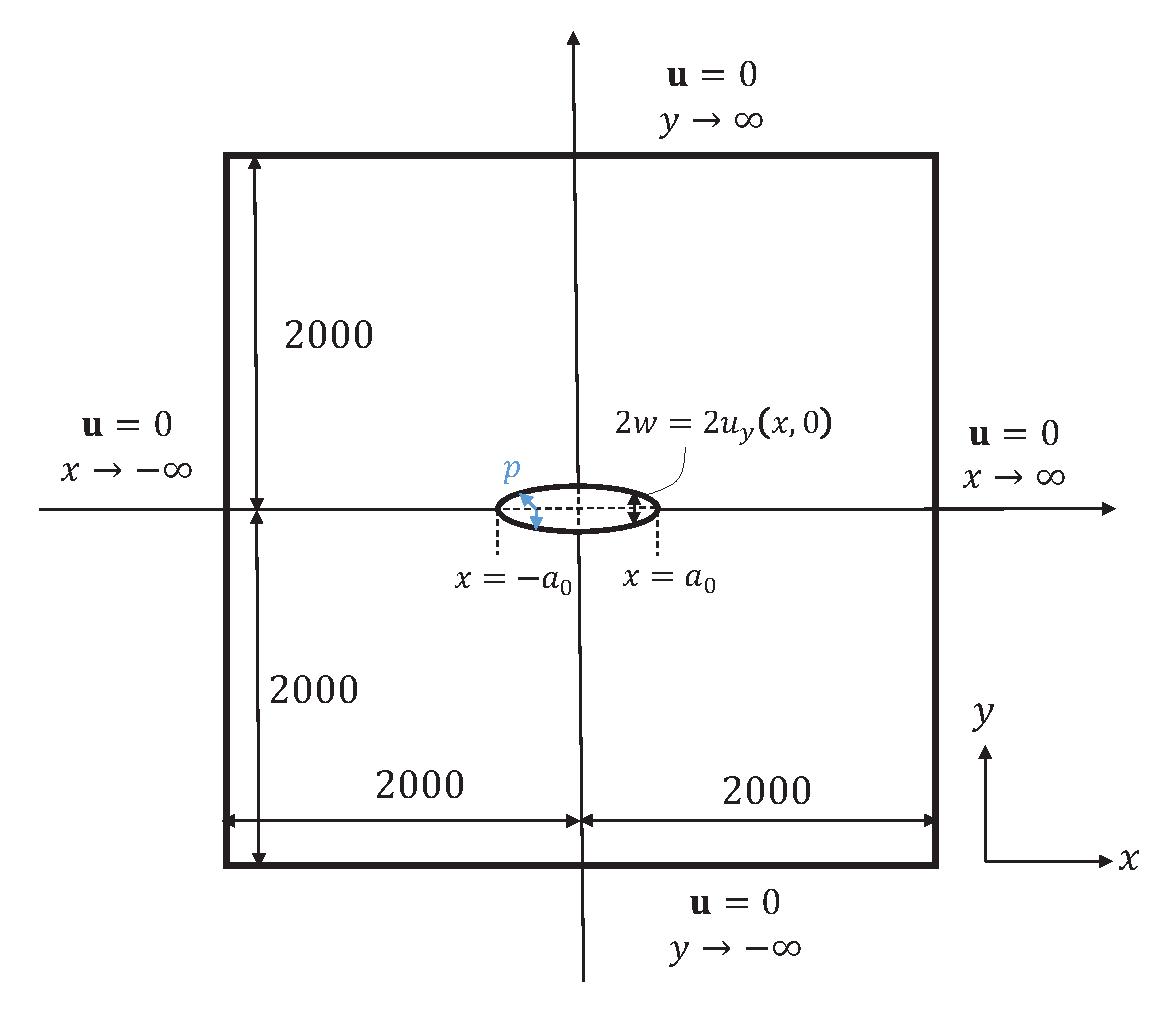
\includegraphics[width=0.8\textwidth]{centerCrack_sneddon.eps}
    \caption{Computation of the crack opening displacement. Schematic view of the deformed line crack in a two dimensional domain.}
    \label{Fig:Sneddon_geometry}
\end{figure}

%\todo{Mostafa: rewrite this part, these two paragraphs are a part of a PhD theses. \cite{Chukwudozie-2016a}}
 
%\paragraph*{Sneddon's 2D benchmark with constant pressure.}  This section simulates the deformation of a static line crack in an infinite two dimensional domain. This is the classic problem solved by Sneddon and Lowengrub (1969). The material is composed of a homogeneous isotropic. The domain is under plain strain conditions and the boundary conditions on the material is such that displacement and stresses vanish at infinity while the crack surface is acted upon by a uniform pressure p.  For the condition where the crack is found in the region defined by $y = 0$, $-l_0\le x \le l_0$, Sneddon and Lowengrub (1969) derived the following analytical expression for the crack opening displacement in the y-direction.
%\begin{equation} \label{eq: sneddon_opening}
%u_y(x,0)= \dfrac{2(p-\sigma_0) l_0}{E'}\sqrt{1-\dfrac{x_0}{l_0}}
%\end{equation}
%where $E'=\dfrac{E}{1-\nu^2}$. The fracture displacement profile is elliptic as evident from Equation \eqref{eq: sneddon_opening}. Thus, the fracture
%\begin{equation*}
% V_f=\pi \dfrac{2(p-\sigma_0) l_0^2}{E'}
%\end{equation*}

%\paragraph*{Compute the fracture width and volume.}  
Bourdin \emph{et al.}~\cite{BourdinCFRAC13} proposed a formula to compute the fracture aperture as:
\begin{equation*}
    w=\mathbf{u}\cdot n_{\Gamma} \simeq \int_{s} \mathbf{u} \cdot \nabla d \, dx.
\end{equation*}
Then, the fracture volume is calculated by integrating the fracture aperture along the fracture's path:
\begin{equation*}
    V_f= \int_{\Gamma} w \, ds \simeq \int_{\Omega} \mathbf{u} \cdot \nabla d \, d\Omega.
\end{equation*}

Figure \ref{Fig:Sneddon_opening} shows the {aperture} profile for different $h$ and $\ell$. The dash line in black represents the Sneddon's analytical solution \cite{SneddonLowengrub69}. Also, the crack volume computed by Sneddon's analytical solution and our numerical tests are summarized in Table \ref{Tab:Sneddon_volume}. %\todo{YS: Any conclusion?}

\begin{figure}[htbp]
    \centering
    \subfloat[]{
    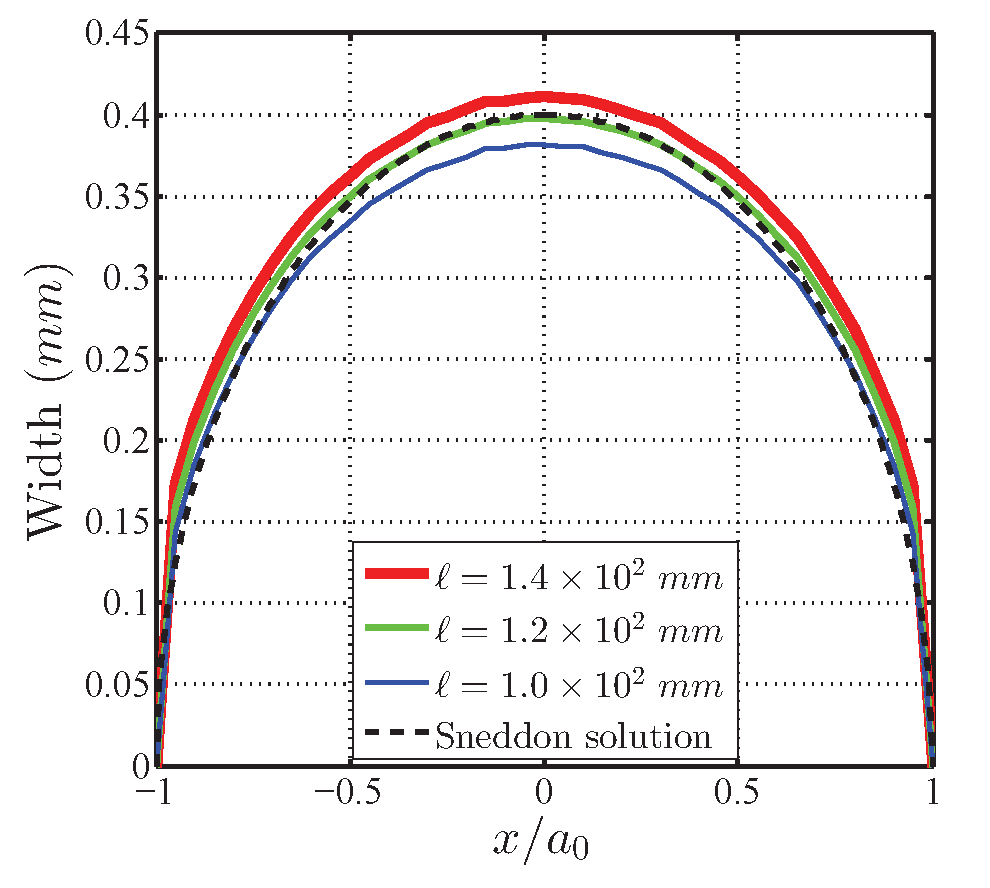
\includegraphics[width=0.5\textwidth]{width_ellVary.eps}
    \label{Fig:Sneddon_opening_ell}}
    \subfloat[]{
    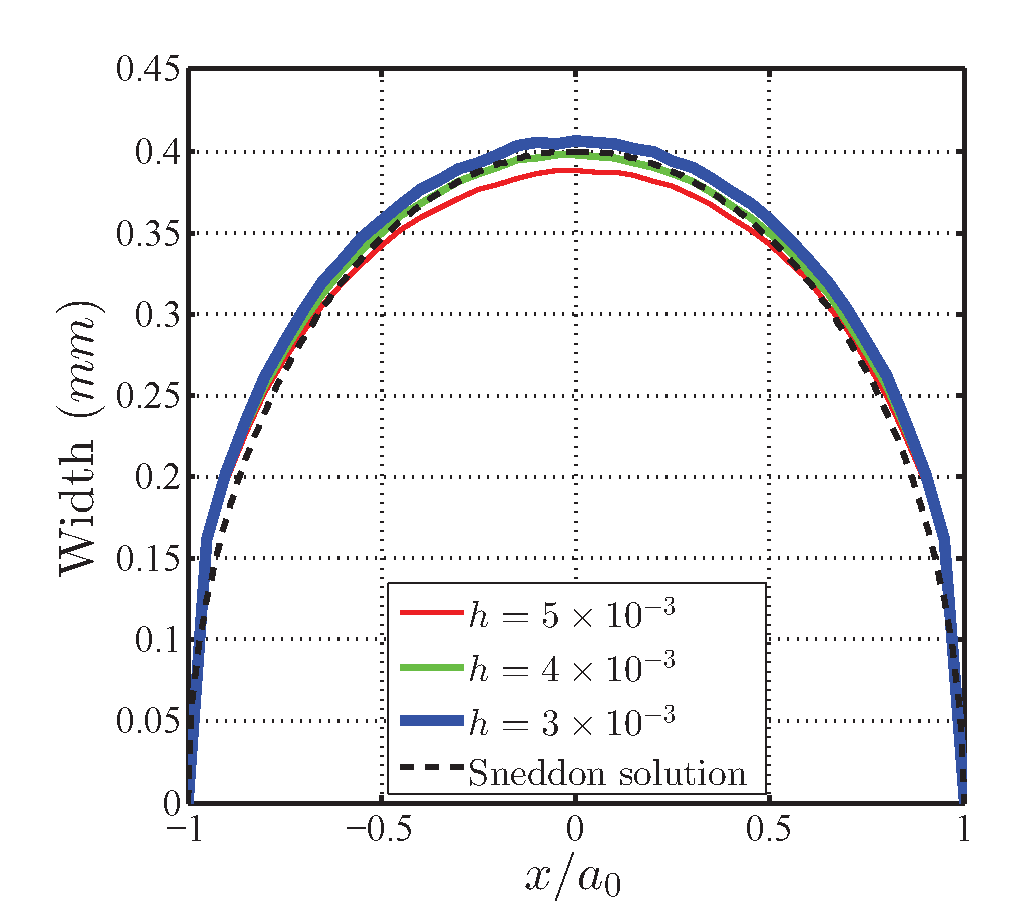
\includegraphics[width=0.5\textwidth]{width_hVary.eps}
    \label{Fig:Sneddon_opening_h}}    
    \caption{Computation of the crack opening displacement. We output the results for (\ref{Fig:Sneddon_opening_ell}) various $\ell$ with $h=4$ mm and (\ref{Fig:Sneddon_opening_h}) various $h$ with $\ell=1.2\times 10^{2}$ mm, and compare them with Sneddon's analytical solution \cite{SneddonLowengrub69}.}
    \label{Fig:Sneddon_opening}
\end{figure}

%\begin{figure}[htbp]
   % \centering
   % \includegraphics[width=0.7\textwidth]{centerCrackOpening.eps}
   % \caption{Phase field profile for center pressurized fracture, where $h=5  \times 10^-3~ \text{mm}$ and $\ell=4h$. }
 %   \label{Fig:opening_Pressrized_fracture_i}
%\end{figure}

\begin{table}[]
    \centering
    \caption{Crack volumes for different $\ell$ for numerical tests and analytical solution ($h=4\text{mm}$).}
    \begin{tabular}{l  c c c}
    \hline 
         $\ell$ (mm)  &1.4$\times 10^{2}$ & 1.2$\times 10^{2}$ &1.0$\times 10^{2}$\\
    \hline 
         Numerical fracture volume (mm$^2$) & 2.89$\times 10^{2}$ & 2.75$\times 10^{2}$  & 2.60$\times 10^{2}$\\
         Analytical fracture volume (mm$^2$) &2.51$\times 10^{2}$\\
    \hline      
    \end{tabular}
    \label{Tab:Sneddon_volume}
\end{table}